\documentclass[12pt]{article}  
 
\usepackage{times,fancyhdr,lastpage}
 \usepackage[a4paper, margin=1in]{geometry}
\usepackage{amsmath,amssymb,enumerate,amsbsy,amsthm,graphicx,titlesec,color}

 \linespread{1.5}
\pagestyle{fancy}

        
  
% Set No indentation
\setlength\parindent{0pt}

% Environments
\theoremstyle{definition}
\newtheorem{theorem}{Theorem}[section]
\newtheorem{proposition}[theorem]{Proposition}
\newtheorem{lemma}[theorem]{Lemma}
\newtheorem{corollary}[theorem]{Corollary}
\newtheorem{definition}[theorem]{Definition}
\newtheorem{example}[theorem]{Example}
\newtheorem{conjecture}[theorem]{Conjecture}
\newtheorem{xca}[theorem]{Exercise}
\newtheorem{remark}[theorem]{Remark}
 \numberwithin{equation}{section}
 
\titleformat{\section}
  {\normalfont\Large\bfseries }{\textbf{Section \thesection}\;\;}
  {0em}{}
  
   \cfoot{\fontsize{11pt}{11pt}\selectfont{Page \thepage\ of \pageref{LastPage}}}
  
  
  \newcommand{\shorttitle}{Distibution of Primes} %A shorter title of the report. It appears as left header.
  
  
\begin{document}

\lhead{\shorttitle}
\rhead{202109/MAT410} %academic session and course code

%Title Page
\begin{titlepage}
\centering
\begin{figure}[h]
  \centering
  
\includegraphics[scale=1 ]{xmumlogo}
  \end{figure}

	 
	
	\vspace{3cm}
	 
	{\huge\bfseries Distribution of Primes\par} %Full title of the report, use all capital letters
	\vspace{4cm}
	{\large  TEO LEE PENG} %Your name, use all capital letters
	
	{\large  MAM2010003} %Your student ID, use all capital letter
	\vfill
	 

% Bottom of the page
	{\large \today\par}

 \end{titlepage}
 
\vfill\pagebreak
 
\tableofcontents                     % automatically generate and include a table of contents

\vfill\pagebreak
%Start each section on a new page 

 

 
 
\section{Introduction}

 

The level of English writing in a report must be appropriate. 
Attention should be paid to correct spelling, grammar, punctuation, sentence structure and clarity of style.

Normally, the word `I' should not be used.

Here are some examples on how to cite papers and books. There are a journal paper \cite{einstein}, 
followed by two journal papers \cite{crank47,Kato1987}, and a book \cite{dirac}. 

\noindent
The following shows how to use list.
\begin{enumerate}[(a)]
\item Students should do individual projects.  

 

 

\item The report must be typed using Latex. The main text should be at least 20 pages, and preferably not more than 50 pages, with font size 12 and 1.5 line spacing. Title page, table of contents and references are not counted.
\end{enumerate}
 
 
 The following shows nested lists. 
 \begin{enumerate}[1.]
 \item The followings are examples of how to include tables.

\begin{enumerate}[(i)]
\item Table 1

\begin{table}[h]
  \centering
    \begin{tabular}{| l c r |r|}
    \hline
    1 & 2 & 3 & 4\\
    \hline
    5 & 6 & 7 & 9 \\
    \hline
    10 & 11 & 12 & 13 \\
    \hline
    \end{tabular}
  \caption{A simple table v1} \label{c1.T.simpletable}
\end{table}


\vfill\pagebreak
\item Table 2


\begin{table}[h]
  \centering
    \begin{tabular}{|| l c r  r||}
    \hline
    \hline
    1 & 2 & 3 & 4\\
    \hline
    5 & 6 & 7 & 9 \\
    \hline
    10 & 11 & 12 & 13 \\
    \hline
    \hline
    \end{tabular}
    
  \caption{A simple table v2} \label{c2.T.simpletable}
\end{table}

\end{enumerate}

\item The following is an example of figure.
\begin{figure}[h]
  \centering
  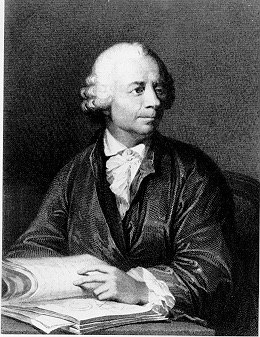
\includegraphics[scale=0.3 ]{euler}
  \caption{A picture of Euler.} \label{c1.F.Euler}
\end{figure}
\end{enumerate}

 
 \vfill\pagebreak
 
\section{Equations}
Different templates for equations.

\begin{enumerate}[(a)]
\item Using “\$\$”.

$$x=x'\cos\theta-y'\sin\theta,\quad
y=x'\sin\theta+y'\cos\theta.$$

\item Using “align”.
\begin{align*} 
x=&x'\cos\theta-y'\sin\theta,\\
y=&x'\sin\theta+y'\cos\theta.\end{align*}



\item Using “equation”. You can use alignment tab by adding “split” environment. 
\begin{equation}\label{eq1}
\begin{split}x=&x'\cos\theta-y'\sin\theta,\\
y=&x'\sin\theta+y'\cos\theta.
\end{split}
\end{equation}The equation \eqref{eq1} is standard.


\item Using “gather”. Each line will automatically centered. You can use alignment tab by adding “split” environment. 
\begin{gather*}
\begin{split}x=&x'\cos\theta-y'\sin\theta,\\
y=&x'\sin\theta+y'\cos\theta.
\end{split}\\
x=x'\cos\theta-y'\sin\theta,\\
y=x'\sin\theta+y'\cos\theta.
\end{gather*}

 
\end{enumerate}
 
 \vfill\pagebreak %Start a new section on a new page
\section{Sections}

If a section contains more than one topic, you need to organize them into   subsections.

 

\subsection{Title of the subsection}

\begin{definition}
	Statement of the definition.
\end{definition}

\begin{theorem}\label{thm.1}[Theorem in Logic]\leavevmode
%leave a line blank

The followings are equivalent.	 
\begin{enumerate}[(a)]
\item $p$ implies $q$.
\item not $q$ implies not $p$.
\end{enumerate}
\end{theorem}

\begin{lemma}
	Statement of the lemma.
\end{lemma}

\begin{corollary}
	Statement of the corollary.
\end{corollary}

\begin{proof}
	Proof of the collary.
	
	This follows from the equation
	\begin{equation}\label{eq2}
	E=mc^2.\end{equation}
\end{proof}


\begin{proof}[Proof of Theorem \ref{thm.1}]
	Proof of Theorem \ref{thm.1}.
	
	This can be proved by consider the following cases.
\end{proof}

\begin{remark}
You need to give explanations to your steps. Use formal language. Do not include symbols like $\Rightarrow$ in your writings. 
\end{remark}

 \vfill\pagebreak



 





 
\appendix
%\include{appendix}
%%------------------------------------------------------------------------------------------------------------------------
% begin of appendix
%%------------------------------------------------------------------------------------------------------------------------
\section{Title for Appendix A}

This is Appendix A. 
%%------------------------------------------------------------------------------------------------------------------------
% end of appendix
%%------------------------------------------------------------------------------------------------------------------------











\vfill\pagebreak

%Start bibliography on a new page.

 
\bibliography{refs}   %refs.bib is the bibliography database
\bibliographystyle{alpha} % alphabetical style

\end{document}

